\chapter{User sessions}
\section{Prototypes - Theis}
In order to get some information from the users about how the user interface should be like we made some sessions with different purpose and users. For the user sessions we made four prototypes, the prototypes is as follows.

\subsection{Hub low fidelity}
This prototype is use in the participatory design session. The prototype is basically just a box with an aluminium sheet as front, this should act like the hub, then we printed some pictures of different types of components, such as bottoms, LEDs and screens. This make it easy to rearrange the design just by moving the pictures. This is a low fidelity prototype because it do not do anything functional, it is just to show the design.
\subsection{Hub high fidelity}
This prototype was made before we had the participatory design session. This was how we have defined his needs, and how we think it should look like. The prototype is also used in the participatory design. We made it with the same box as the low fidelity hub prototype, we used a mbed to control some LEDs in the front sheet. This is a high fidelity prototype, because it can show how the hub will react on different actions, it gives the user the same experience as a fully operation hub with this interface would do.
\subsection{Power point mid fidelity}
This prototype is used in the first usability test. It is an interactive power point with slides to show the different web pages, we have said that this is a mid fidelity prototype, it gives the user a good experience as the final page would do, but it dose not have any dynamic data, it is all static so that it is just to see how the interaction with the page works.
\begin{figure}[h!]
	\center
		\setlength\fboxsep{0pt}
		\setlength\fboxrule{1pt}
		\fbox{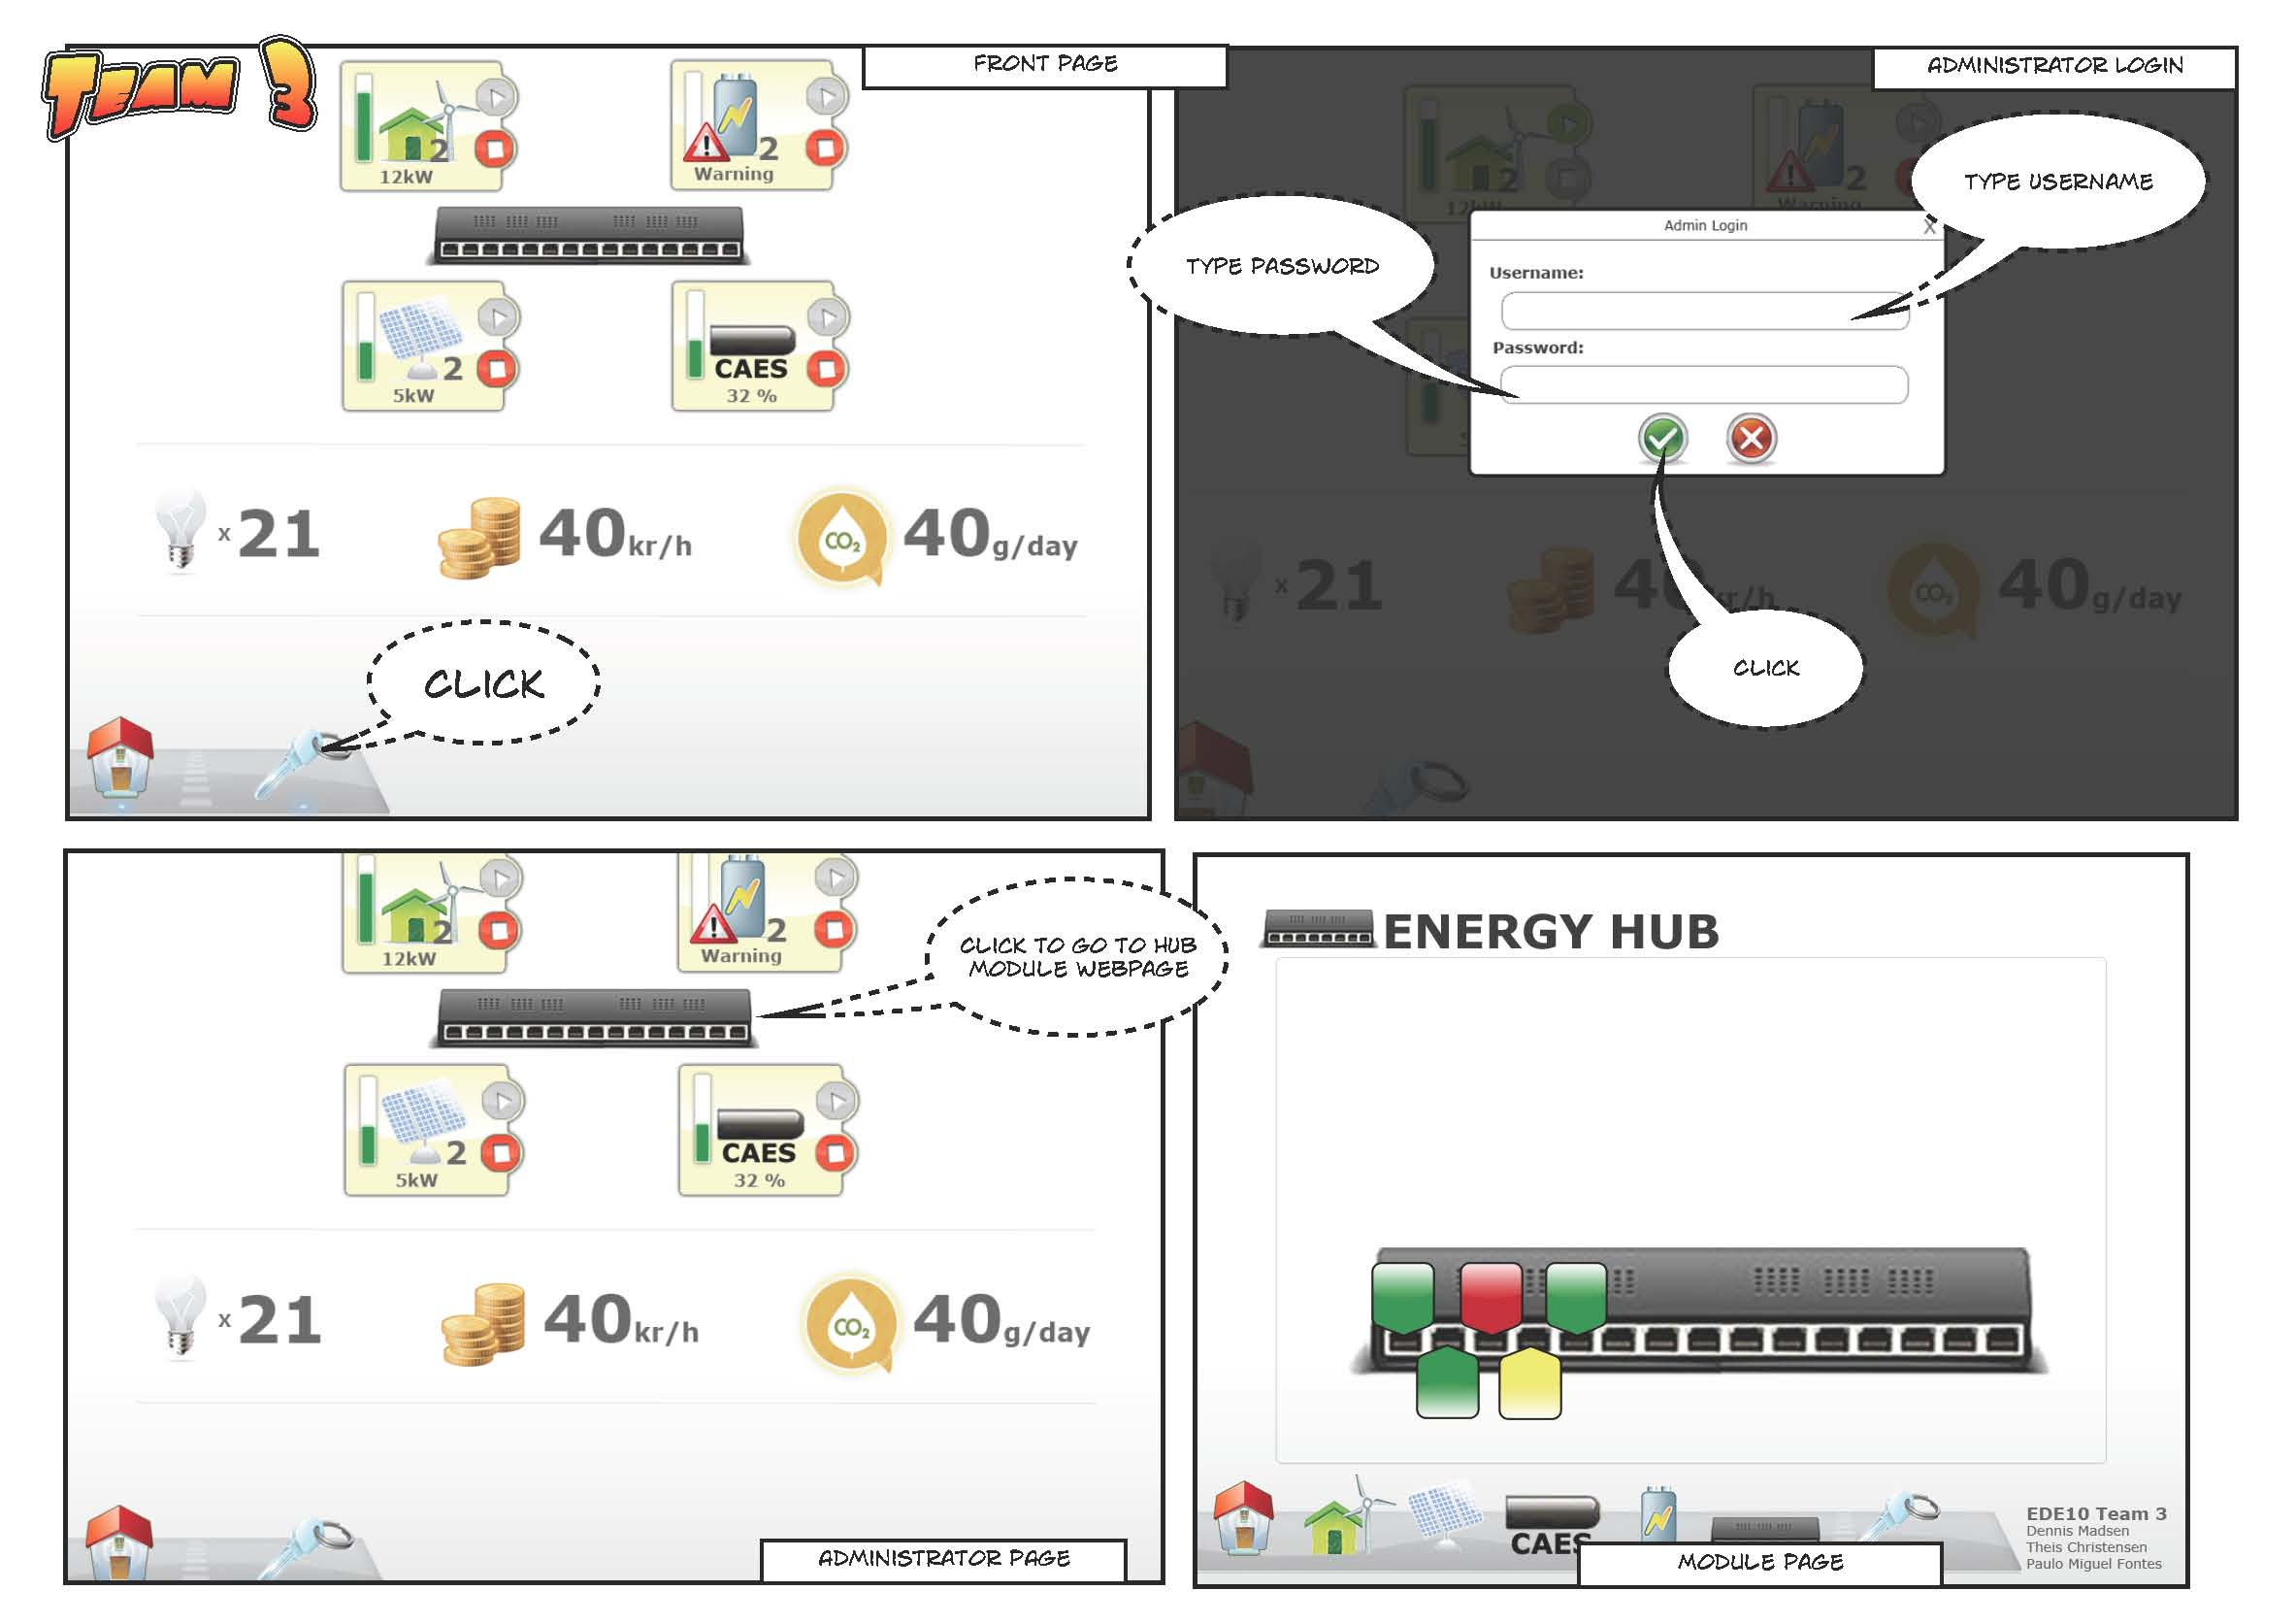
\includegraphics[width=0.4\textwidth]{images/web_interface1.jpg}}
   	\caption{Picture of the power point slides}
   	\label{fig:web_interface1}
\end{figure}
\subsection{HTML web page mid fidelity}
This prototype is used in the second usability test. It is the web page developed in EWEB1 course, the purpose of the site is to give at picture of how the final web page would look like and work. We had said this to be mid fidelity as the power point because it perform the same purpose and have the same functionality.
\begin{figure}[h!]
	\center
		\setlength\fboxsep{0pt}
		\setlength\fboxrule{1pt}
		\fbox{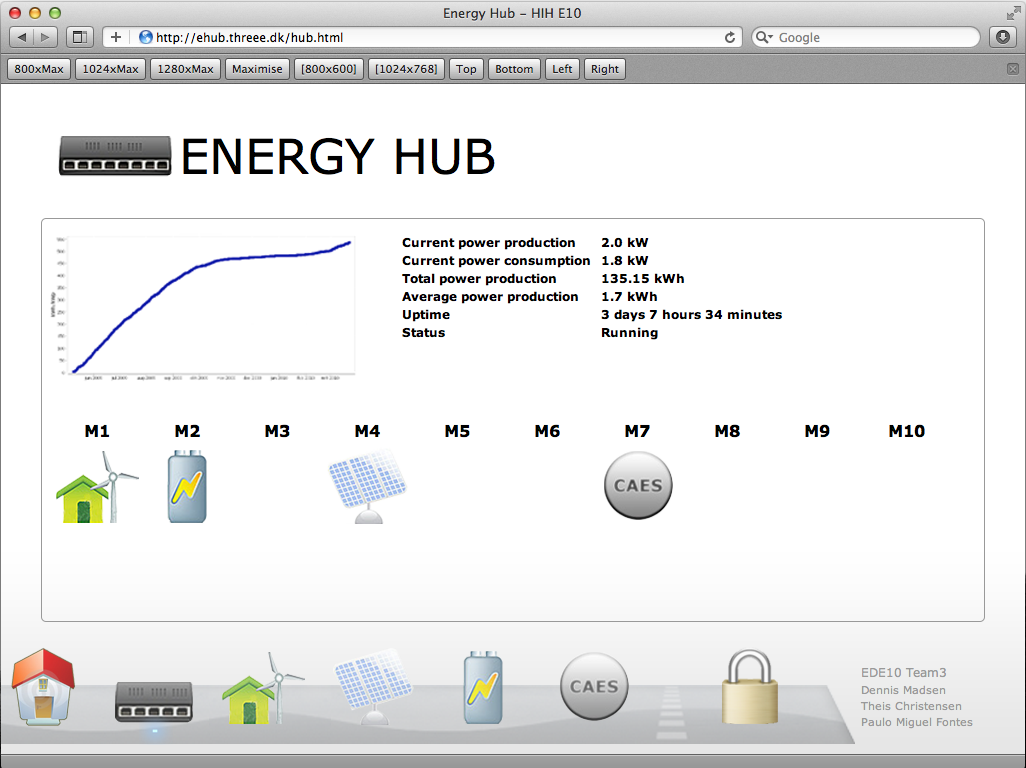
\includegraphics[width=0.4\textwidth]{images/screen_hub_page.png}}
   	\caption{Picture of the hub web page}
   	\label{fig:web_hub_interface}
\end{figure}
\begin{figure}[h!]
	\center
		\setlength\fboxsep{0pt}
		\setlength\fboxrule{1pt}
		\fbox{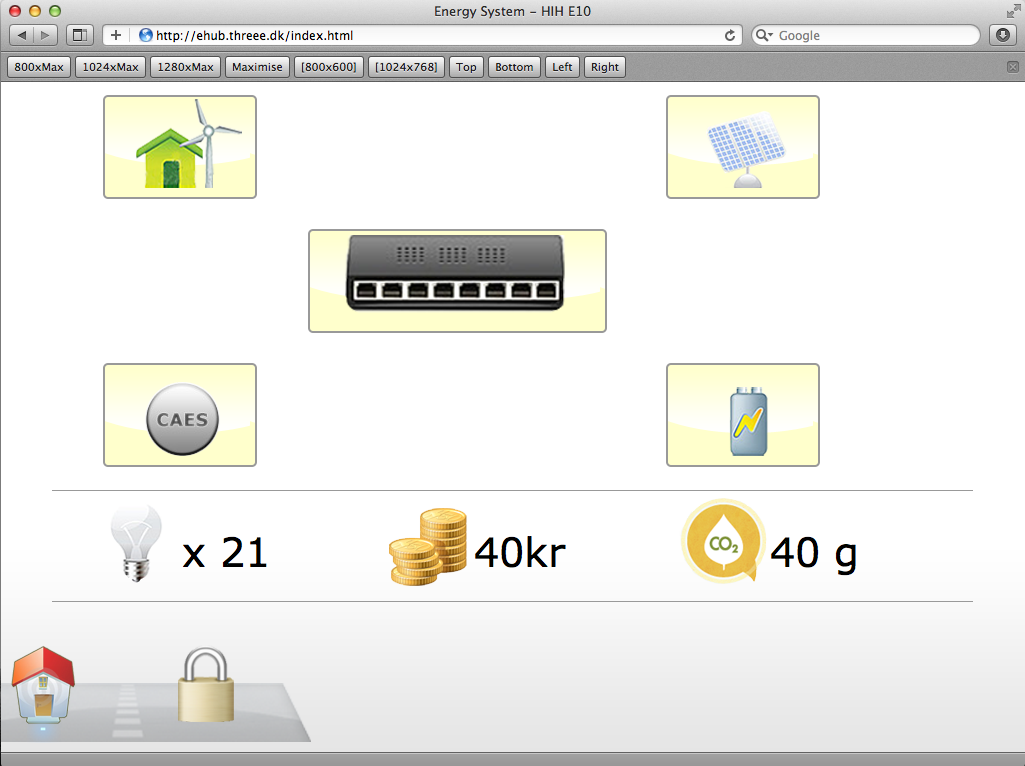
\includegraphics[width=0.4\textwidth]{images/screen_index_page.png}}
   	\caption{Picture of the index web page}
   	\label{fig:web_index_interface}
\end{figure}%%%%%%%%%%%%%%%%%%%%%%%%%%%%%%%%%%%%%%%%%
\section{Participatory Design - Dennis}
As explained earlier, the hub module is divided into two sections, the web interface and the physical interface on the hub. 
The goal of the participatory design session with the customer Jan was to clarify the level of interaction he wants on the hub module, but also where the different things should be placed. A video of the session can be found on the wiki page (find link in the introduction section). Before the session, pictures of small buttons, LED's, screens, connecters etc. were printed out to easy to process of placing components on the front panel. Jan's job was now, with some guidance instructions, to place the components he wanted on the hub and where he wanted them. The design ended up with a clean design containing: 
\begin{itemize}
	\item 1 Power button, to turn on the hub. The button should have built in LED.
	\item 1 emergency button (powers off everything).
	\item 1 on/off switch for each module (position switch).
	\item 2 indication LED for each module (green on = module is powered on. Red on = module is powered off).
	\item A 230VAC plug is placed on the front to connect: light, phone-chargers or similar. 
\end{itemize}
To get access to the front panel of the hub, a locker should be open with a key, to protect agains fiddle-fingers. The emergency button is of cause operational all the time, and no locker needs to be opened to use it.
\\When finishing his idea about the front panel of the hub, Jan was introduced to another solution, which worked as a prototype of the finish product. Jan was asked to go through some tasks:
\begin{itemize}
	\item Turn on the hub.
	\item Connect a module.
	\item Turn on the connected module.
	\item Identify an error on a module.
	\item Repair the module.
	\item Shut down the system.
\end{itemize}
The general impression from Jan was positive, but some of functions found on the interface was unnecessary as he will primarily use a PC to check the status of the different devices (on the web interface). The placement and method of connecting new devices was fine and the same with turning on and off the hub. Instead of the pushbuttons found on the prototype, as mentioned, he wants position switches. The indication of every module was fine, but unnecessary indicators should be removed. 
%%%%%%%%%%%%%%%%%%%%%%%%%%%%%%%%%%%%%%%%%
\section{First usability tests - Theis}
\textbf{How has the setup for these sessions been, and how did they turn out. Did we learn anything???}
In the first usability test we used the power point as a demonstration prototype of the web page. We made the session with Rene as the end user of the web interface to the system. We had a stationary camera behind him, to record the actions on the screen, and a webcam in the computer to record his face expressions. In the session Rene had free hands to play around with the power point.


%%%%%%%%%%%%%%%%%%%%%%%%%%%%%%%%%%%%%%%%%
\section{Second usability tests - Paulo}

In this usability test task were defined and asked for the users to follow, this was made in the new interface and the interface from EDE09, this way we can have a comparison between two different interfaces navigation. Users were timed for each task, is important to know how much time users will take to do each task so we can understand the difficulty of the navigation in our system and what could be change to make it more understandable for the user.
\\
\\Three different individual where selected to this usability test:\\
- Person directly involved on the project.\\
- Person with an overview of the project.\\
- Person without not involved, or overview of the project.\\
\\
5 tasks were asked to the users:\\
- Login as an admin user.\\
- View photovoltaic page.
- See the average power on the energy hub.\\
- Find the current status on the battery module.\\
- Log out.
\\















